\documentclass[twocolumn]{article}

\usepackage{parskip}
\usepackage{titling}
\usepackage{graphicx}
\usepackage[backend=bibtex,
style=numeric
]{biblatex}
\addbibresource{../bibliography}

% Document metadata
\title{
    GEOG 5551 Term Project: Project Paper
}
\author{
    Aamdal, Haakon\\
    \texttt{aamda001@umn.edu}
}


% Margins
\topmargin=-0.45in
\evensidemargin=0in
\oddsidemargin=0in
\textwidth=6.5in
\textheight=9.0in
\headsep=0.25in

\begin{document}
\maketitle

\section{Introduction}
\label{sec:Introduction}
According to a white paper published by Bell Labs \cite{Bell_Labs2013-st} on internet traffic growth, the end-user internet connection traffic demand is forecasted to increase by 3.7 from 2012 to 2017. Nearly all of the demand is forecasted to come from residental and business fixed internet connections. There's over 30 internet service providers (ISPs) in the United States \cite{noauthor_undated-uf}, resulting in a highly competitive market with low margins of profit. This paper explains how an internet service provider (ISP) can take advantage of a geographical information system (GIS) to maximize profit and minimize risk.

The solution proposed in this paper will be a tool for locating the ISP customers with the most potential. A GIS is advantageous for this task, because the ISP would be interested in physical location of businesses and households most likely to sign up for a new fixed internet connection service. In order to find the customers with the most potential, the system will use several attributes of the households and businesses, like the total income/revenue or number of residents/employees. In addition to this, the cost of installing new customers will have to be taken into consideration when ranking profitability and potential. Clustered customers have lower costs per installation. In addition, the closer the customer to existing infrastructure, the better.

\section{Data}
\label{sec:Data}
This project is highly dependent on good data sources to be successful. Data is collected from a number of sources, all listed in this section.

\begin{figure}
  \centering
  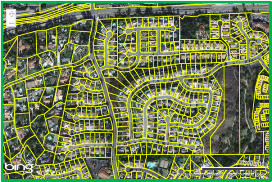
\includegraphics[width=0.45\textwidth]{img/parcel.png}
  \caption{Parcel data from Digital Map Products}
  \label{fig:parcel}

\end{figure}
\paragraph{Parcel data}

\label{par:Parcel data}
A quick google search reveals that there exists several companies that sells parcel data for the United States. Digital Map Products \footnote{http://www.digmap.com/} is one of them. They deliver vector and raster digital parcel boundaries for over 120 million US parcels. The data also contains the assessors parcel number (APN), which makes it possible to link the parcels with tax data. Their vector dataset would be most useful for this application, and can be downloaded in the standard ArcGIS Shapefile format. The dataset is however not free, you need to contact them to get an offer. An example map is shown in Figure~\ref{fig:parcel}.

\begin{figure}
  \centering
  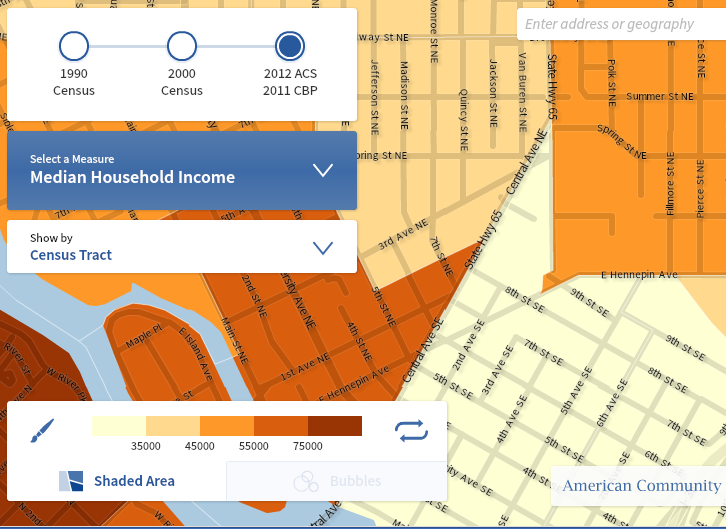
\includegraphics[width=0.45\textwidth]{img/census.png}
  \caption{Median Household Income from the United States Census Bureau for Minneapolis NE. The data is divided by census tracts.}
  \label{fig:census}
\end{figure}
\paragraph{US Census data}
\label{par:Us Census data}
The United States Census Bureau can provide data on several households attributes, including average income, average number of children and precentage of population with high school diploma. Since the US Census only samples a fraction of the total population, and are required to conserve anonymity, their data are divided into census tracts/blocks or even counties. Please see Figure~\ref{fig:census} for an example of how the census tracts are divided. All of the data from the US Census are free of charge.

\begin{figure}
  \centering
  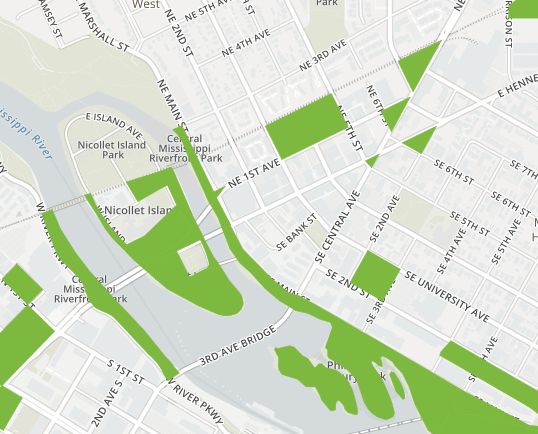
\includegraphics[width=0.45\textwidth]{img/nbm.png}
  \caption{The National Broadband Map showing which areas in Minneapolis NE that only have one or two broadband suppliers.}
  \label{fig:nbm}
\end{figure}
\paragraph{National Broadband Map}
\label{par:National Broadband Map}
The National Broadband Map\footnote{http://www.broadbandmap.gov/} is an updated dataset to where you can search, analyze and map broadband availability across the United states. The data includes broadband speed, broadband technology, number of broadband providers and more. It can map areas where there are fewer broadband suppliers than others. It also contains data which correlates bandwidth speed with demographics, like population density, age, income or education. The National Broadband Map are free of charge.

\begin{figure}
  \centering
  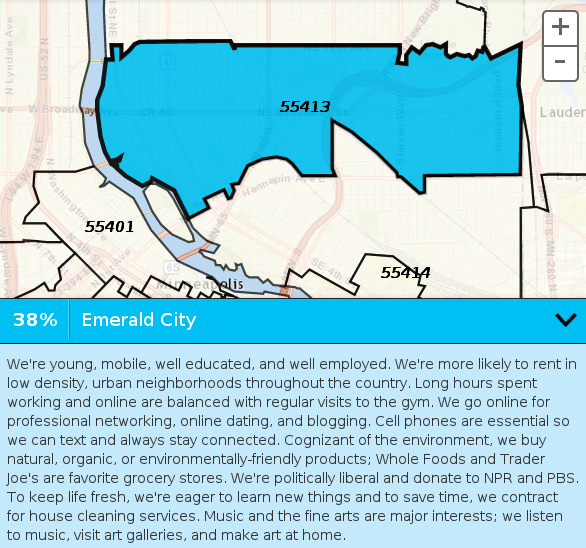
\includegraphics[width=0.45\textwidth]{img/tapestry.png}
  \caption{The Esri Tapestry data for ZIP 55414. The data explains the average citizen of the area, including leisure time activities, political standpoints and buying patterns.}
  \label{fig:tapestry}
\end{figure}
\paragraph{Esri Tapestry Segmentation}
\label{par:Esri Tapestry Segmentation}
Esri provides a dataset named Esri Tapestry Segmentation\footnote{http://www.esri.com/landing-pages/tapestry/} aiming to improve understading of people's lifestyle choices, what they buy and how they spend their free time. The tapestry classifes U.S. residential neighborhoods into 67 unique segments based on socioeconomic and demographic characteristics. Each segment offers a picture of the average citizen, revealing information on leisure activities and buying patterns. See Figure~\ref{fig:tapestry}. The tapestry data is available for purchase from Esri.

\paragraph{Business data}
\label{par:Business data}
The United States Census Bureau also provides data about businesses\footnote{http://www.census.gov/econ/susb/}, which includes number of establishments, employment and annual payroll for most U.S. businesses. This data is very coarse grained, as it is divided into census tracts or counties. A more granular  option is the US Business Locations and Business Summary database\footnote{http://www.esri.com/data/esri\_data/business-overview/business} from Esri. This database gives you the location of all businesses in the United States, as well as relevant attributes like annual sales and number of employees. The business data is available for purchase from Esri and can be downloaded in vector format as points.

\begin{figure}
  \centering
  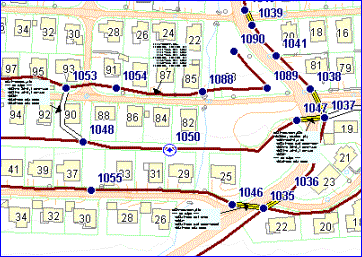
\includegraphics[width=0.45\textwidth]{img/telme.png}
  \caption{Sample documentation from the TelMe software. Different network infrastructure like cables, connections and hubs are documented spatially.}
  \label{fig:telme}
\end{figure}
\paragraph{Existing network infrastructure}
\label{par:Existing network infrastructure}
Another important part is the data of the ISP's existing network infrastructure. At a minimum, the application requires all relevant components, like hubs, connectors and cables, to be documented spatially. This data should be in vector format. There exists several products out there to help documenting cable infrastructure. The TelMe\footnote{https://micado.no/index.php?cont=cont/3TelMe\_TM.html} software from Micado AS is one of them, and an example of spatial documentation is shown in Figure~\ref{fig:telme}.


\subsection{GIS operations for preparing data for analysis}
\label{sub:GIS operations for combining data}
\begin{figure}
  \centering
  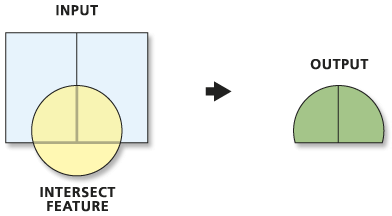
\includegraphics[width=0.45\textwidth]{img/intersect.png}
  \caption{Splitting spatial features and combining attributes. Courtesy of \cite{noauthor_undated-dw}.}
  \label{fig:intersect}
\end{figure}
Since we have data from many different sources, they would need to be combined before starting the analysis. Because we would like to have as fine grained data as possible, we would like our sorce tables to be individual parcels or businesses. We would then have to combine this fine-granularity data with the other data which is more coarse-grained. An easy way of doing this would be to do use the overlay technique Intersect. The result of this would be the coarser grained data split into smaller pieces and combined with the businesses or parcels, effectively expanding the source tables with new attributes. Please see Figure~\ref{fig:intersect} for how the intersect operation works.

It is however very important to be aware of the pitfalls by combining coarse grained information with fine grained. For example, all households would be assigned an average income. However, this income does not reflect the average income of the house, it is still the average income of the census tract the household belongs to. This needs to be taken into consideration when analysing the data. However, if the data sources are split up differently, you will get a tighter classification of each parcel. For intance, you can have two households with the same income (because they are in the same census tract), but have different number of broadband suppliers, because the National Broadband Map splits up its blocks differently that the US Census.


The ISPs network infrastructure might not be documented spatially. Depending on the format of the current documentation, getting the required vector data might include:
\begin{itemize}
  \item If the network is documented on paper maps with drawing and sketches, these maps would need to be scanned and georeferenced. Since we need vector data, manual digitizing of relevant map features like boxes, cables and connectors might need to be digitized/extracted manually.
  \item If the network is documented non-spatially, like in a spreadsheet, all relevant points would have to be geocoded. The documentation might already include coordinates. This would require us to convert the aspatial table to a spatial one using the x and y attributes. If the documentation does not coordinates, but rather addresses, we could look these addresses up and put each point into the map based on the result. Getting the cables into the map would require some logical analysis of where to find the endpoints. Once found, cables could be drawn as lines in the map between the already geocoded points.
\end{itemize}


\section{Potential and profitability}
\label{sec:Potential and profitability}
Even with a wide range of data available, it's not obvious how to use them. This section will aim to explain which attributes that might be relevant for ranking new customers in terms of potential and profitability.

\subsection{Household potential}
\label{sub:Potential}

\paragraph{Analyzing data from the Broadband Network Map}
\label{sub:Analyzing data from the Broadband Network Map}
The \textit{National Broadband Map} provides a map showing the correlation between broadband speed and demographics data, more specifically for population density, age, income and education. By visually inspecting the map with the different categories, one can come up with the following conclusions:
\begin{itemize}
  \item Median age does not correlate with the broadband speeds. 
  \item Median income correlates to broadband speeds. The higher the income, the higher speed.
  \item The precentage of people with high school diploma correlates to broadband speed.
\end{itemize}
Even though this visual inspection is not very accurate, it still pinpoints attributes worth looking at when looking for customers that would like to improve it's internet connection.

\paragraph{Internet usage}
\label{sub:Internet usage}
The \textit{PewResearch Internet Project} provides data about U.S. internet usage \cite{noauthor_2013-ev}. Although this statistics does not explicitly state the type of connection (speed, fixed vs. mobile), it's still a valid guideline for pointing out users with high potential. The report backs up the observation from Section \ref{sub:Analyzing data from the Broadband Network Map}: The more eductated and well paid population got more potential. In addition to this, the statistic also shows that the younger the population, the higher internet usage.

\paragraph{The Esri Tapestry Segmentation}
\label{sub:The Esri Tapestry Segmentation}
One could also use the Esri Tapestry Segmentation directly. This data provides a definition of each customer segment. All segment descriptions could be analysed with broadband connection demand in mind. For instance, the ISP could look for customer segments describing people with a high use of internet traffic intensive applications like gaming and streaming.

\subsection{Business potential}
\label{sub:Businesses}
The research for project have not been able to find any sources on business potential whet it comes to broadband connections. One could still normal intuition to do a profitiability assessment. The more employees, the higher demand for a good internet connection. In addition, high yearly revenue will also be an indicator of purchasing power.

\subsection{Profitability}
\label{sub:Profitability}
The cost of installing the new customers will also have to be taken into consideration when ranking profitability and potential. According to a paper on economics of fibre to the home by Weldon, M. K. and Zane, F. \cite{Weldon2003-xq}, the population density of the area will affect the total cost. More specifically, the lower population density, the higher the cost of the new network infrastructure. In other words, potential customers clustered together with other potential customers is will be cheaper to install. Additionally, the paper states that labor costs for digging down the cables in a trench (trenching) is a big part of the expenses, so proximity to already existing network infrastructure should be considered when finding new customers.
Even though the customers are potential and have high purchasing power, they might not be profitable due to other considerations.

Another aspect of customer profitability is the precence of other broadband providers in the area. If the households or businesses are ranked as very potential customers, it's very likely some other ISPs already supply broadband connections to them. Expanding the network in that area would be associated with high risk. It's not very likely that the customers would like to change a broadband supplier they're already satisfied with, and more so paying the initial cost of installing a new connection. The competitors network documentation are normally classified. Luckily, whe have access to the data from the National Broadband Map. Areas with none or few providers can be ranked higher than areas with much competition, as well as areas with lower speed and old technology.

\section{Methods, data presentation and analysis}
\label{sec:Methods}
Paragraph about why we don't want to do more now, and let the operator do the most.



\paragraph{Representing potential}
\label{par:Representing potetnial}


Could also use a score. This would require careful analysis of how to weight the different stuff. A relevant discussion about this is included later in the section

\paragraph{Filtering areas with many competitors}
\label{par:Filtering areas with many competitors}
same as above

\paragraph{Close to current infrastructure}
\label{par:Close to current infrastructure}

\paragraph{Finding clustered customers}
\label{par:Finding clustered customers}
K-means, heatmap.



We have all our relevant attributes and know what to look for. 


\section{Risk assesment and potential pitfalls}
\label{sec:Risk assesment and potential pitfalls}


\section{Conclusion}
\label{sec:Conclusion}

\printbibliography

\end{document}
